\documentclass[tikz,border=6pt]{standalone}
\usepackage[T1]{fontenc}
\usepackage{lmodern}
\usetikzlibrary{arrows.meta,positioning}
\definecolor{ink}{HTML}{1F2933}
\definecolor{ext}{HTML}{FFF3BF}
\definecolor{bar}{HTML}{DBE4FF}
\definecolor{mid}{HTML}{FFE8CC}
\begin{document}
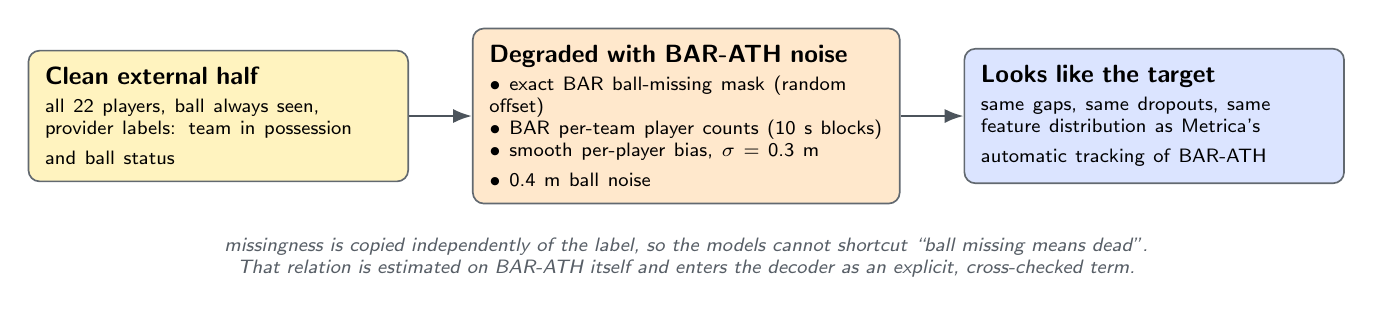
\begin{tikzpicture}[font=\sffamily\small, node distance=8mm,
  box/.style={draw=ink!70, rounded corners=4pt, align=left, text width=44mm, inner sep=6pt, line width=0.6pt},
  arr/.style={-{Latex[length=2.4mm]}, line width=0.9pt, draw=ink!80}]
\node[box, fill=ext] (clean) {\textbf{Clean external half}\\[2pt]\scriptsize all 22 players, ball always seen,\\ provider labels: team in possession\\ and ball status};
\node[box, fill=mid, right=of clean, text width=50mm] (noise) {\textbf{Degraded with BAR-ATH noise}\\[2pt]\scriptsize $\bullet$ exact BAR ball-missing mask (random offset)\\ $\bullet$ BAR per-team player counts (10 s blocks)\\ $\bullet$ smooth per-player bias, $\sigma$ = 0.3 m\\ $\bullet$ 0.4 m ball noise};
\node[box, fill=bar, right=of noise] (target) {\textbf{Looks like the target}\\[2pt]\scriptsize same gaps, same dropouts, same\\ feature distribution as Metrica's\\ automatic tracking of BAR-ATH};
\draw[arr] (clean) -- (noise);
\draw[arr] (noise) -- (target);
\node[below=3mm of noise, font=\sffamily\scriptsize\itshape, text=ink!75, align=center, text width=130mm]
 {missingness is copied independently of the label, so the models cannot shortcut ``ball missing means dead''.\\ That relation is estimated on BAR-ATH itself and enters the decoder as an explicit, cross-checked term.};
\end{tikzpicture}
\end{document}
